%% For submission and review of your manuscript please change the
%% command to \documentclass[manuscript, screen, review]{acmart}.
%%
%% When submitting camera ready or to TAPS, please change the command
%% to \documentclass[sigconf]{acmart} or whichever template is required
%% for your publication.
\documentclass[sigconf]{acmart}

\RequirePackage{xeCJK} % 使用xeCJK宏包支持中文

%%
%% \BibTeX command to typeset BibTeX logo in the docs
\AtBeginDocument{%
  \providecommand\BibTeX{{%
    Bib\TeX}}}

%% Rights management information.  This information is sent to you
%% when you complete the rights form.  These commands have SAMPLE
%% values in them; it is your responsibility as an author to replace
%% the commands and values with those provided to you when you
%% complete the rights form.
\setcopyright{acmlicensed}
\copyrightyear{2018}
\acmYear{2018}
\acmDOI{XXXXXXX.XXXXXXX}
%% These commands are for a PROCEEDINGS abstract or paper.
\acmConference[Conference acronym 'XX]{Make sure to enter the correct
  conference title from your rights confirmation email}{June 03--05,
  2018}{Woodstock, NY}
%%
%%  Uncomment \acmBooktitle if the title of the proceedings is different
%%  from ``Proceedings of ...''!
%%
%%\acmBooktitle{Woodstock '18: ACM Symposium on Neural Gaze Detection,
%%  June 03--05, 2018, Woodstock, NY}
\acmISBN{978-1-4503-XXXX-X/2018/06}


%%
%% Submission ID.
%% Use this when submitting an article to a sponsored event. You'll
%% receive a unique submission ID from the organizers
%% of the event, and this ID should be used as the parameter to this command.
%%\acmSubmissionID{123-A56-BU3}

%%
%% For managing citations, it is recommended to use bibliography
%% files in BibTeX format.
%%
%% You can then either use BibTeX with the ACM-Reference-Format style,
%% or BibLaTeX with the acmnumeric or acmauthoryear sytles, that include
%% support for advanced citation of software artefact from the
%% biblatex-software package, also separately available on CTAN.
%%
%% Look at the sample-*-biblatex.tex files for templates showcasing
%% the biblatex styles.
%%

%%
%% The majority of ACM publications use numbered citations and
%% references.  The command \citestyle{authoryear} switches to the
%% "author year" style.
%%
%% If you are preparing content for an event
%% sponsored by ACM SIGGRAPH, you must use the "author year" style of
%% citations and references.
%% Uncommenting
%% the next command will enable that style.
%%\citestyle{acmauthoryear}


%%
%% end of the preamble, start of the body of the document source.
\begin{document}

%%
%% The "title" command has an optional parameter,
%% allowing the author to define a "short title" to be used in page headers.
\title{EDMIT:交互式运动辅导中增强决策能力的端到端智能框架}

%%
%% The "author" command and its associated commands are used to define
%% the authors and their affiliations.
%% Of note is the shared affiliation of the first two authors, and the
%% "authornote" and "authornotemark" commands
%% used to denote shared contribution to the research.
\author{Jinhua Du}

\email{dujh22@mails.tsinghua.edu.cn}
\orcid{0009-0008-4170-6452}
\affiliation{
  \institution{Tsinghua University}
  \city{Beijing}
  \country{China}
}

\author{Mufeng Xing}
\author{Ziheng Zhou}
\author{Ruilin Zhang}
\affiliation{
  \institution{Banlan Technology}
  \city{Suzhou}
  \country{China}
}

\author{Zexun Jiang}
\affiliation{
  \institution{School of Data Science and Intelligent Media Communication University of China,}
  \city{Beijing}
  \country{China}
}

%%
%% By default, the full list of authors will be used in the page
%% headers. Often, this list is too long, and will overlap
%% other information printed in the page headers. This command allows
%% the author to define a more concise list
%% of authors' names for this purpose.
% \renewcommand{\shortauthors}{Trovato et al.}

%%
%% The abstract is a short summary of the work to be presented in the
%% article.
\begin{abstract}
一对一辅导行之有效,但现有基于大模型的教学产品在多轮互动与人机共演中仍难以实现个体化决策。我们聚焦三项问题:如何以低成本从稀缺且非结构化的教练经验构建可用数据;如何设计在互动过程中自适应覆盖个体差异的反馈机制;以及基于 AI 的运动辅导是否能达到甚至超越人类教练。为此,我们提出 EDMIT——面向交互式运动辅导的端到端智能体框架:从教练行为轨迹出发构建“种子→增广”的数据管线,提出标准化决策本体与可执行决策链,并以闭环反馈在会话中自适应调节提示粒度、练习难度与纠错策略。我们实现原型并开展双盲受控研究(10 名用户、10 名教练),在不知来源条件下与提示词式基线比较。结果显示,EDMIT 与人类教练的决策一致性更高,显著提升用户满意度与认可度,并达到同类方法的 SOTA 水平,表明智能体驱动的人机共演可有效弥合个性化运动辅导中的决策缺口,并为未来 AI 教练系统设计提供实证依据与方法学启示。
\end{abstract}

%%
%% The code below is generated by the tool at http://dl.acm.org/ccs.cfm.
%% Please copy and paste the code instead of the example below.
%%
\begin{CCSXML}
  <ccs2012>
  <concept>
  <concept_id>10003120.10003121.10003122.10003332</concept_id>
  <concept_desc>Human-centered computing~User models</concept_desc>
  <concept_significance>500</concept_significance>
  </concept>
  </ccs2012>
\end{CCSXML}

\ccsdesc[500]{Human-centered computing~User models}

%%
%% Keywords. The author(s) should pick words that accurately describe
%% the work being presented. Separate the keywords with commas.
\keywords{交互式运动辅导, 智能体框架, 个性化决策, 大型语言模型(LLM), 数据增广, 反馈闭环, 决策链, 双盲实验, 实证研究}
%% A "teaser" image appears between the author and affiliation
%% information and the body of the document, and typically spans the
%% page.
\begin{teaserfigure}
  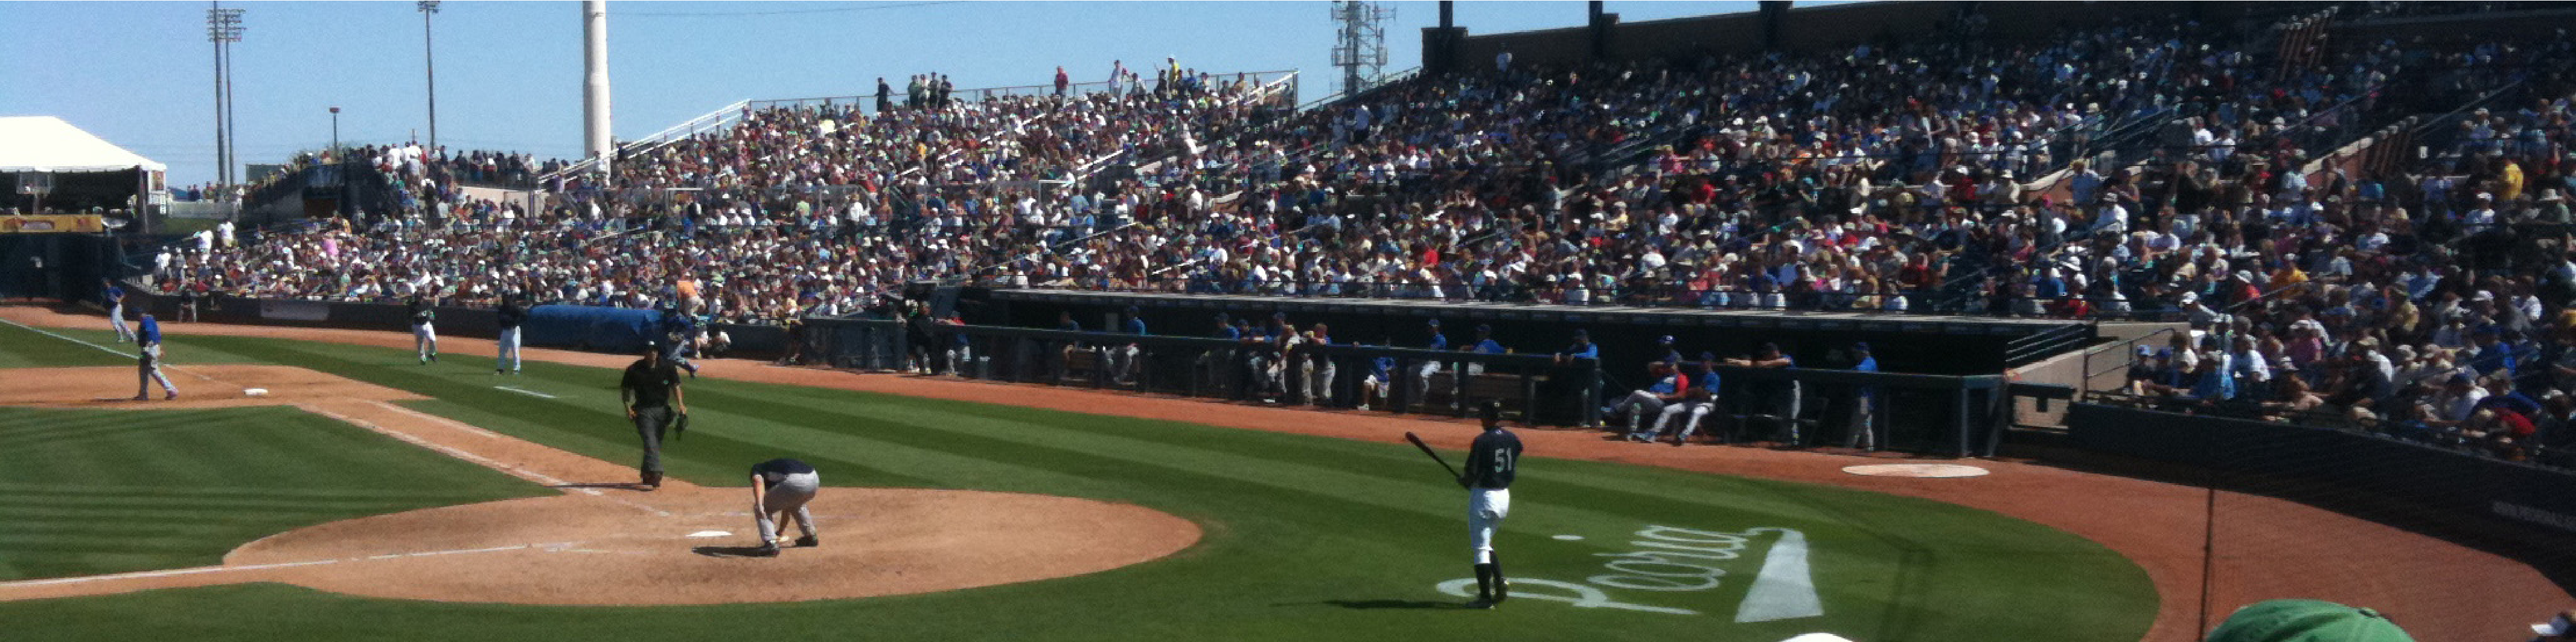
\includegraphics[width=\textwidth]{sampleteaser}
  \caption{Seattle Mariners at Spring Training, 2010.}
  \Description{Enjoying the baseball game from the third-base
  seats. Ichiro Suzuki preparing to bat.}
  \label{fig:teaser}
\end{teaserfigure}

% \received{20 February 2007}
% \received[revised]{12 March 2009}
% \received[accepted]{5 June 2009}

%%
%% This command processes the author and affiliation and title
%% information and builds the first part of the formatted document.
\maketitle

\section{Introduction}
一对一的人类辅导已被证明是一种非常有效的教学形式\cite{chiLearningHumanTutoring2001}。随着人工智能领域的快速发展特别是基于大型语言模型的相关技术成熟,涌现出诸多服务于用户的智能系统,包括教育\cite{wangLargeLanguageModels2024}、医疗\cite{heSurveyLargeLanguage2025}和体育科学\cite{connorLargeLanguageModels2023}等。自从以o1\cite{openaiOpenAIO1System2024a}和deepseek\cite{deepseek-aiDeepSeekR1IncentivizingReasoning2025b}为代表的深度推理模型出现,智能系统的推理能力显著增强,已经在数学\cite{chenDeepMathCreativeBenchmarkEvaluating2025}、代码\cite{jainLiveCodeBenchHolisticContamination2024}等领域达到人类博士生水平。

尽管取得这些进展,但在用户使用大模型教学产品,过程中仍面临重大挑战:“个性化决策缺失”。造成该问题的原因在于:常见的智能辅助系统主要以AI模型作为算法基础,并通过固定的提示词构建智能问答系统\cite{goldbachIntelligentTutoringSystems2020,kwonBIPEDPedagogicallyInformed2024}。单一的提示词和模型本身限制了系统决策适配人机交互过程中由人提出的个性化需求,而且其一次性生成的特性使其在涉及多轮交互与连续决策的场景中难以发挥作用,因此固有的方法并不能有效应对复杂的辅助教学场景。

以辅助运动辅导场景为例,虽然人类教练在教学过程中:能够针对不同的用户情况进行个性化决策,但是使用虚拟教练往往无法简单复刻真实教练的能力。既是因为人类教练的经验往往没有形成固定的文本数据方便模型训练,而且相关数据量不足,也难以完全覆盖多样化的场景需要。因此目前仍没有用户体验较好的交互式运动辅助系统。

为弥补这一空白,在运动辅助领域解决“个性化决策缺失”的问题,我们提出了一个端到端的智能体框架EDMIT,用于交互式运动辅导中增强AI系统的决策能力,最大程度模拟学习人类教练进行运动交互指导中的决策行为。具体而言,通过我们以用户为中心的研究,我们试图回答三个问题:

\begin{itemize}
  \item {\texttt{研究问题1}}: 如何设计一个全自动的自主AI系统,从非常有限的非结构化人类教练经验中,用较低的成本完成系统必要的数据工程输入。
  \item {\texttt{研究问题2}}: 如何设计一个有效的决策增强系统,以支持在交互式运动中自适应地覆盖用户多样化、个性化的运动辅导需求。
  \item {\texttt{研究问题3}}: 基于AI的运动辅助系统是否能够有效模拟人类教练进行指导,是否有超过人类教练的可能?或者说,基于AI的运动辅助系统的智能上限在哪里?
\end{itemize}

基于对真实教练指导用户的行为轨迹建模与数据采集,我们构造了种子训练数据与评测数据集。在种子训练数据上开发了一个数据增广框架,将种子训练数据扩展到任意尺度,以覆盖构造智能AI系统的数据需要(研究问题1);通过借鉴人类运动学习中的“反馈闭环理念”,我们标准化建模了在辅助运动辅导场景下所有可能的决策节点,并系统化构造出完整的智能决策链,通过智能体驱动整个决策链的具体执行,自适应地为多样化、个性化用户提供运动辅导服务(研究问题2)。

为评估基于EDMIT框架是否能真正帮助用户提升其运动水平,我们首创性地在AI运动辅助领域引入“双盲实验”。我们开发了一个采用EDMIT的原型系统来为真实用户提供服务,用户事先无法确认服务来源是真实教练还是虚拟教练,并在辅助教学结束后为多个方案进行打分。我们通过对10名真实用户和10名真实教练进行受控用户研究,比较了EDMIT和真实教练的一致性,以及和其他传统方法的性能差异(研究问题3)。结果表明,EDMIT框架能提供人类教练水平的决策能力,达到已有方法中的SOTA水平,显著增强用户对AI辅助运动产品的认可度和满意度。

总之,我们的研究探索了一个交互式运动辅导中增强决策能力的端到端智能框架,以弥合人类教练经验和AI系统的智能差距,从而提升用户的运动学习效果。我们的贡献体现在四个方面:1)一个复杂系统框架,给出了交互式运动辅导中增强决策能力的方法论;2)一个开源系统,提供框架对应的代码实例和产品,支持后续研究;3)一项用户研究, 评估了我们的AI系统设计对用户的有效性;4)为设计未来AI驱动的交互式运动辅助系统提供了见解,旨在实现个性化辅助运动教学中有效的人机交互。

\section{Related Work}

\subsection{AI辅助决策}

大模型
专用于AI辅助决策的相关方法

【tutoring system】医疗:1. DDxTutor: Clinical Reasoning Tutoring System with Differential Diagnosis-Based Structured Reasoning 

\subsection{AI驱动的交互式运动辅导}

AI在交互式运动中的运动实例、开源方法or 系统

\section{Methods}

框架:四个决策点(need 决策点的输入)

周期性决策:
交互单元(组间) 组间做组内决策
临时性决策:
临时交互行为(组内)

\section{Experiments}

\section{Results}

\section{Discussion}






\begin{acks}
在致谢部分,应注明资金来源和其他支持,并向协助研究和论文撰写的个人及团体致谢。致谢部分应置于文档参考文献部分之前。
\end{acks}

%%
%% The next two lines define the bibliography style to be used, and
%% the bibliography file.
\bibliographystyle{ACM-Reference-Format}
\bibliography{sample-base}


%%
%% If your work has an appendix, this is the place to put it.
\appendix

\section{Research Methods}


\end{document}
\endinput
%%
%% End of file `sample-sigconf-xelatex.tex'.
